\documentclass[journal]{IEEEtran}
\usepackage[a5paper, margin=10mm, onecolumn]{geometry}
\usepackage{lmodern}
\usepackage{tfrupee}
\setlength{\headheight}{1cm}
\setlength{\headsep}{0mm}

\usepackage{gvv-book}
\usepackage{gvv}
\usepackage{cite}
\usepackage{amsmath,amssymb,amsfonts,amsthm}
\usepackage{algorithmic}
\usepackage{graphicx}
\usepackage{textcomp}
\usepackage{xcolor}
\usepackage{txfonts}
\usepackage{listings}
\usepackage{enumitem}
\usepackage{mathtools}
\usepackage{gensymb}
\usepackage{comment}
\usepackage[breaklinks=true]{hyperref}
\usepackage{tkz-euclide}
\usepackage{listings}
\def\inputGnumericTable{}
\usepackage[latin1]{inputenc}
\usepackage{color}
\usepackage{array}
\usepackage{longtable}
\usepackage{calc}
\usepackage{multirow}
\usepackage{hhline}
\usepackage{ifthen}
\usepackage{lscape}
\usepackage{xparse}

\bibliographystyle{IEEEtran}

\title{12.264}
\author{EE25BTECH11043 - Nishid Khandagre} % Replace with your name

\begin{document}
\maketitle

\renewcommand{\thefigure}{\theenumi}
\renewcommand{\thetable}{\theenumi}

\numberwithin{equation}{enumi}
\numberwithin{figure}{enumi}

\textbf{Question}:\
Consider the system of equations
\begin{align*}
2x_1 + x_2 + x_3 &= 0 \\
x_2 - x_3 &= 0 \\
x_1 + x_2 &= 0
\end{align*}
This system has
\begin{itemize}
\item a) a unique solution
\item b) no solution
\item c) infinite number of solutions
\item d) five solutions
\end{itemize}

\textbf{Solution: }

    \begin{align}
    \vec{A}\vec{x} = \vec{0}
    \end{align}
    \begin{align}
    \vec{A} =\myvec{
    2 & 1 & 1 \\
    0 & 1 & -1 \\
    1 & 1 & 0
    }
    \end{align}
    \begin{align}
    \vec{x} =
    \myvec{
    x_1 \\ x_2 \\ x_3
    }
    \end{align}
    
Augmented matrix:
\begin{align}
    \myvec{
    2 & 1 & 1 & \vrule & 0 \\
    0 & 1 & -1 & \vrule & 0 \\
    1 & 1 & 0 & \vrule & 0
   }
\end{align}
    $R_1 \rightarrow \frac{1}{2}R_1$
    \begin{align}
    \myvec{
    1 & 0.5 & 0.5 & \vrule & 0 \\
    0 & 1 & -1 & \vrule & 0 \\
    1 & 1 & 0 & \vrule & 0
    }
    \end{align}
    $R_3 \rightarrow R_3 - R_1$
    
   \begin{align}
    \myvec{
    1 & 0.5 & 0.5 & \vrule & 0 \\
    0 & 1 & -1 & \vrule & 0 \\
    0 & 0.5 & -0.5 & \vrule & 0
    }
    \end{align}

    $R_3 \rightarrow R_3 - 0.5 R_2$
    \begin{align}
    \myvec{
    1 & 0.5 & 0.5 & \vrule & 0 \\
    0 & 1 & -1 & \vrule & 0 \\
    0 & 0 & 0 & \vrule & 0
    }
    \end{align}

    \begin{align}
    x_1 + 0.5x_2 + 0.5x_3 &= 0 \\
    x_2 - x_3 &= 0
    \end{align}
    \begin{align}
    x_2 = x_3
    \end{align}
    Substitute into the first equation:
    \begin{align}
    x_1 + 0.5x_2 + 0.5x_2 &= 0 \\
    x_1 + x_2 &= 0 \\
    x_1 &= -x_2
    \end{align}
    Let $x_2 = t$. Then $x_3 = t$, and $x_1 = -t$.
    \begin{align}
    \myvec{x_1 \\ x_2 \\ x_3} = t \myvec{-1 \\ 1 \\ 1}, \quad t \in \mathbb{R}
    \end{align}
Since there is one free parameter $t$, the system has infinitely many solutions.\\
Also rank(A) $<$ 3, and the system is consistent (it has solutions) therefore the system has infinitely many solutions.
The answer is option(c).

\begin{figure}[H]
\centering
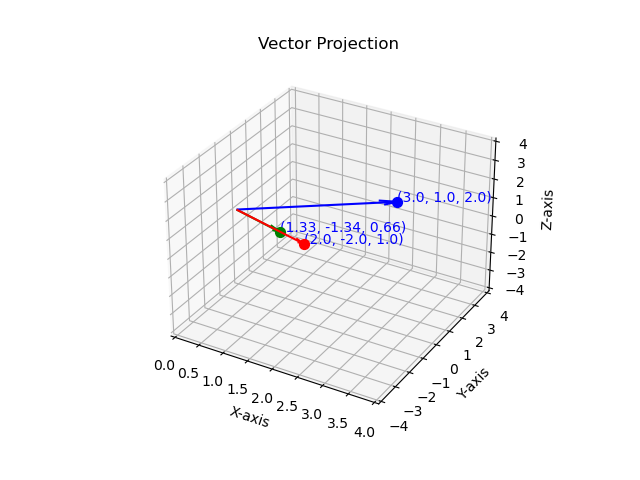
\includegraphics[width=0.7\columnwidth]{fig1.png}
\caption{}
\label{fig:1}
\end{figure}

\end{document}